\documentclass[conference]{IEEEtran}
\usepackage{cite}
\usepackage{adjustbox}
\usepackage{amsmath,amssymb,amsfonts}
\usepackage{algorithmic}
\usepackage{graphicx}
\usepackage{textcomp}
\usepackage{xcolor}
\usepackage[table]{xcolor}
\def\BibTeX{{\rm B\kern-.05em{\sc i\kern-.025em b}\kern-.08em
    T\kern-.1667em\lower.7ex\hbox{E}\kern-.125emX}}
\begin{document}

\title{Project: COVID-19 Assisted Diagnosis\\


\author{\IEEEauthorblockN{Carlo Heemeryck\textsuperscript{1}}
\and
\IEEEauthorblockN{Willem Van Nieuwenhuyse\textsuperscript{1}}
\and
\IEEEauthorblockN{Seppe Vanrietvelde\textsuperscript{2}}
\and
\IEEEauthorblockN{Luca Visser\textsuperscript{2}}
\and

\textsuperscript{1} Bachelor of Science in de ingenieurswetenschappen - werktuigkunde-elektrotechniek \hfill\\
\textsuperscript{2} Master of Science in Statistical Data Analysis - Computational Statistics\hfill\\}
}
\maketitle



\section{Introduction}
Adds context to your project (referencing the material in your bibliography is important~\cite{b1, b2}) and presents the content of the following sections (starting with Section~\ref{sec:task_1}).

Includes tables with quantitative results (Table~\ref{table:example}) and images (Fig.~\ref{fig:example}) from your project while carefully explaining their meaning and how you produced them.
\begin{table}[htbp]
\caption{Table Type Styles}
\begin{center}
\begin{tabular}{|c|c|c|c|}
\hline
\textbf{Table}&\multicolumn{3}{|c|}{\textbf{Table Column Head}} \\
\cline{2-4} 
\textbf{Head} & \textbf{\textit{Table column subhead}}& \textbf{\textit{Subhead}}& \textbf{\textit{Subhead}} \\
\hline
copy& More table copy$^{\mathrm{a}}$& &  \\
\hline
\multicolumn{4}{l}{$^{\mathrm{a}}$Sample of a Table footnote.}
\end{tabular}
\label{table:example}
\end{center}
\end{table}

\begin{figure}[htbp]
\centerline{
\includegraphics{Images/fig1.png}}
\caption{Example of a figure caption.}
\label{fig:example}
\end{figure}






\section{Task 1: Data Exploration, Pre-Processing and Augmentation}\label{sec:task_1}

\subsection{Loading the data}
The grayscale chest X-ray images are loaded at their original resolution of 299 × 299 pixels. The labels, either COVID or NORMAL, are taken from the folder names containing the images and assumed to be accurate. From the outset, the dataset was pre-divided into training (1,600 images), validation (400 images), and test (200 images) sets. This original distribution is preserved for the exercise, with an additional combined training and validation set comprising 2,000 images.

\subsection{Data exploration}
Exploration consists of checking the shape of the data, evaluating the distribution of the two classes, plotting a few examples and checking pixel and global average and standard deviation. This is replicated for training, validation and test datasets and serves as an initial look at the data and to possibly detect problems at an early stage in the project.
All the images in the training dataset are of the same size and there are an equal amount in both classes, which is good. A few labeled examples are given in figure \ref{fig:example_images}.

\begin{figure}[htbp]
\centerline{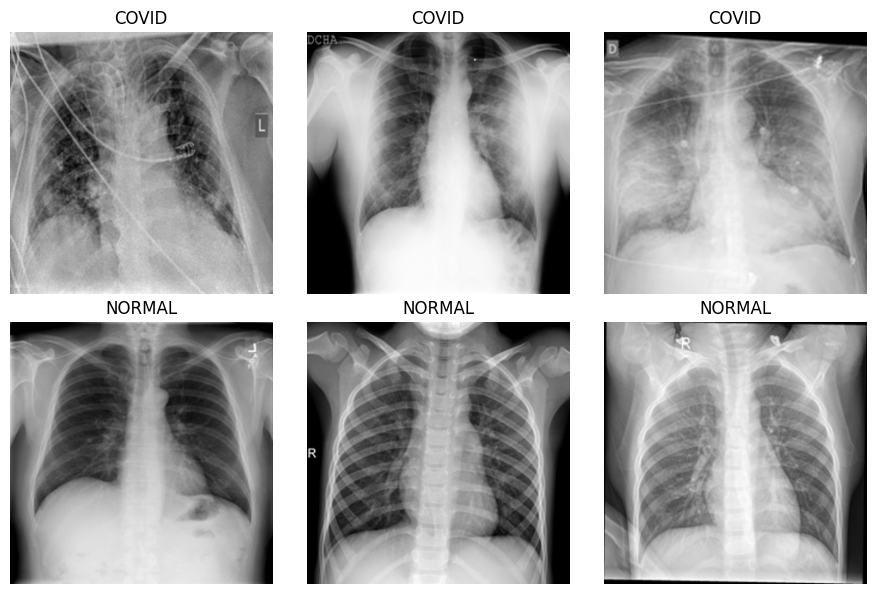
\includegraphics[width=\linewidth]{Images/example_images.png}}
\caption{A few images from the training dataset with accompanying labels.}
\label{fig:example_images}
\end{figure}

There seem to be no clear differences between the NORMAL and COVID images. However, the limitation to grayscale images, low contrasts, different zoom levels and slight variations in angles could be problems for classification. Also if there are, to us unrecognisable, artifacts in mostly one category, generalization to new images could be problematic.
Over all images in the training dataset the average value and the standard deviation at every pixel location can be visualized to show a sort of average image and a heatmap for variation. These visualizations, together with the average and standard deviation of all pixels, are given in figure \ref{fig:pixel_statistics}.

\begin{figure}[htbp]
\centerline{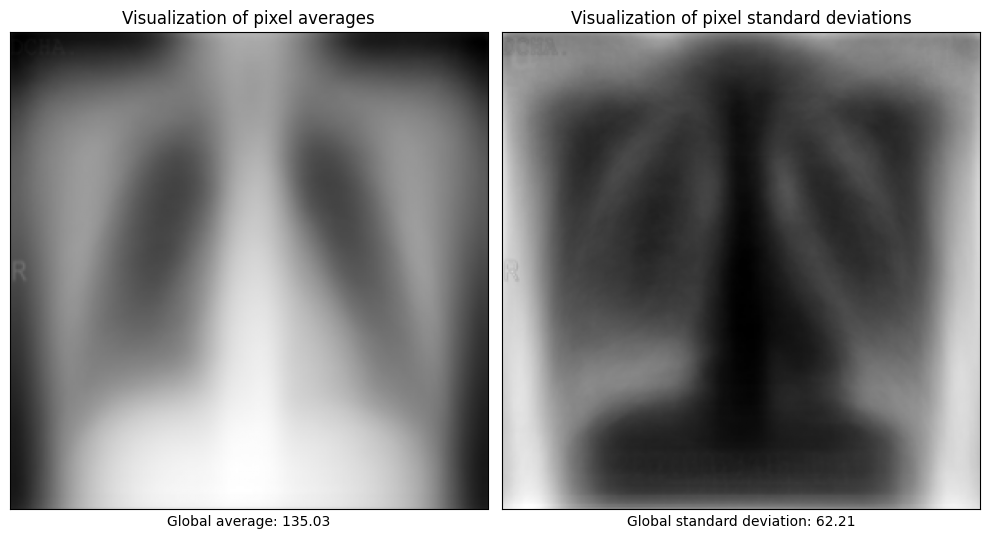
\includegraphics[width=\linewidth]{Images/pixel_statistics.png}}
\caption{A visualization of the average image (left) and a variation heatmap (right) with accompanying global statistics from the training dataset.}
\label{fig:pixel_statistics}
\end{figure}

Replicating all this for the validation and test datasets give very comparable results, indicating that the images were uniformly divided over the different sets. The exploration of the validation and test sets can be consulted in the notebook.

\subsection{Pre-processing}
Next, some pre-processing steps are implemented and evaluated, namely down sampling to 128 x 128 pixels using bilinear interpolation and a few normalization strategies. The result of down sampling, given in figure \ref{fig:downsample}, is still recognisable to the human eye. As such, it is assumed that the model still gets enough information from this. Implementing this down sampling strategy should reduce training time while not losing too much performance.

\begin{figure}[htbp]
\centerline{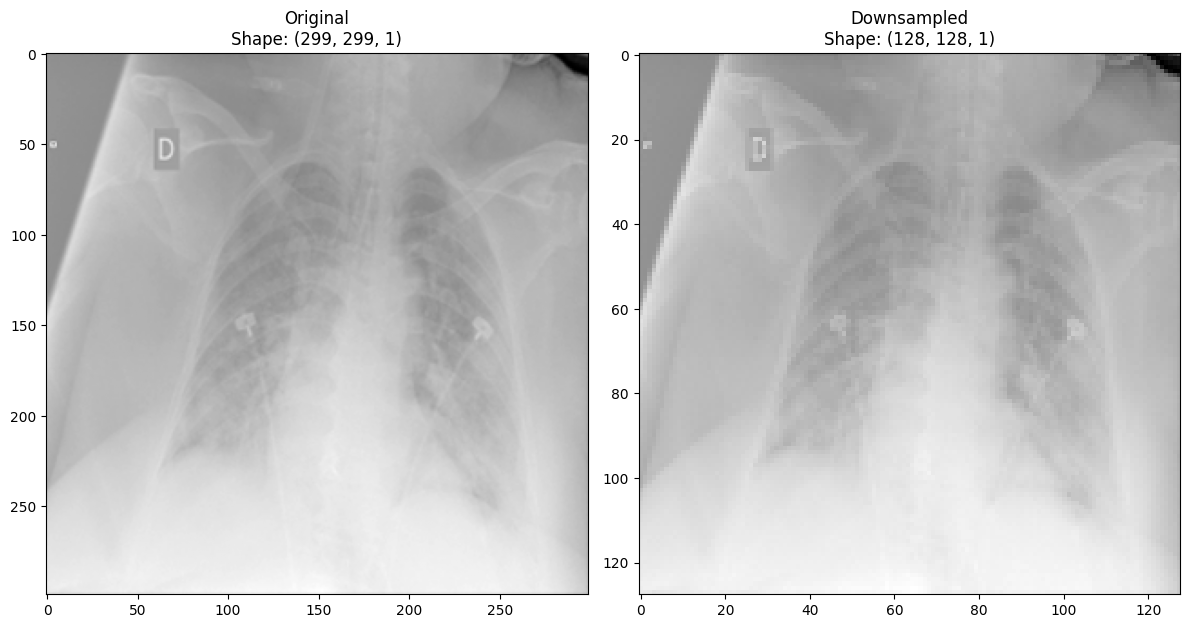
\includegraphics[width=\linewidth]{Images/downsample.png}}
\caption{An example of a downsampled image using bilinear interpolation (299x299 -> 128x128).}
\label{fig:downsample}
\end{figure}

Normalization through the use of a fixed value (dividing by 255), sample statistics (subtracting the overall mean and dividing by the overall standard deviation of the current sample (training, validation or test)) and statistics of the training dataset (subtracting the overall mean and dividing by the overall standard deviation of the training dataset) were tried out. All of these strategies resulted in visually the same image but with pixel values with a far lower magnitude. However, normalizing using training set-wide image statistics (mean and std) and applying the same normalization across all images is the most correct method as it causes no data leakage. Normalization based on the training dataset will thus be used in the project.  

\subsection{Augmentation}
Finally, based on the variety of the plotted images a few augmentation strategies are implemented, namely randomly altering the brightness and the contrast by a factor between 0.6 and 1.4 and randomly rotating the images (anti)clockwise up to 30°. Examples of these augmentation are given in figure \ref{fig:augmentation}.

\begin{figure}[htbp]
\centerline{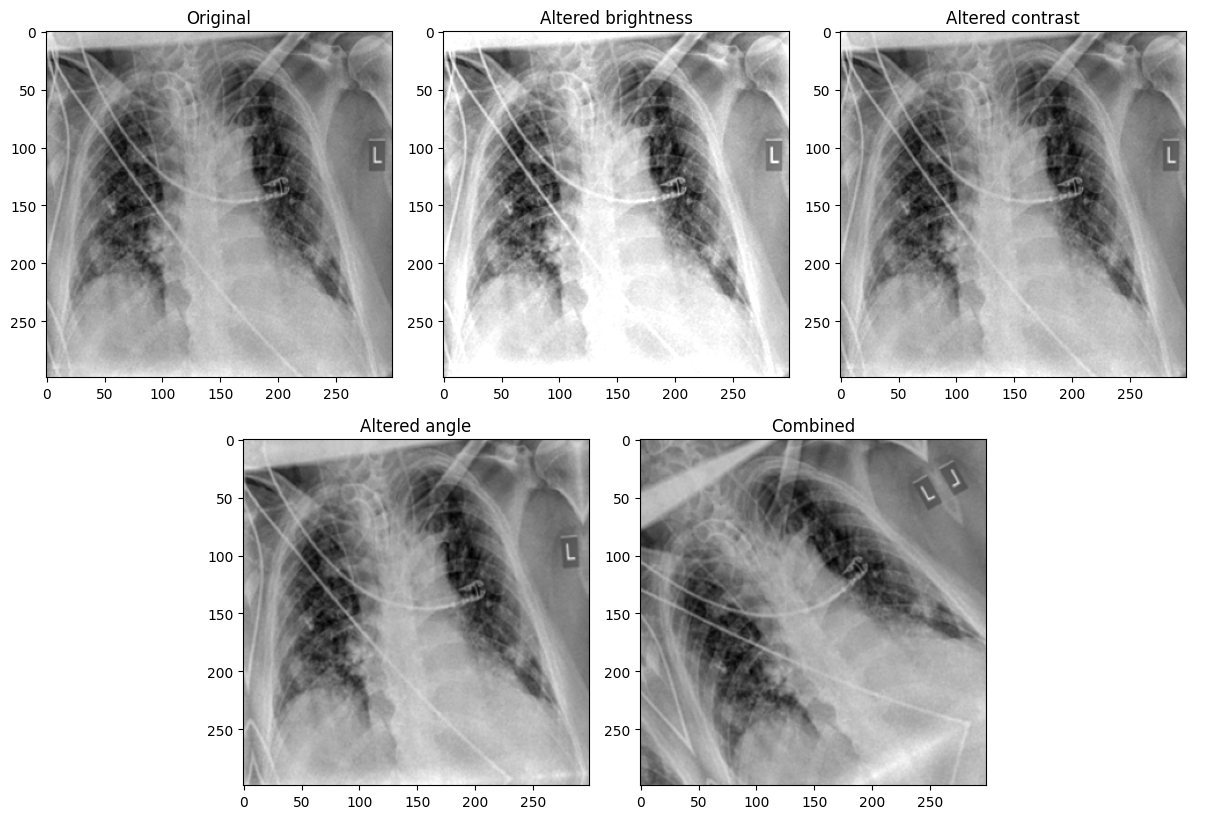
\includegraphics[width=\linewidth]{Images/augmentation.png}}
\caption{Examples of different transformations as well as the combination of them together.}
\label{fig:augmentation}
\end{figure}

Augmentation should only result in images that could occur in test/unseen data. Based on the data we have, intense augmentation doesn't seem al that necessary. It will thus only be considered if necessary.

\subsection{Pipeline}
A pipeline consisting of loading the images correctly, with optional downsampling, followed by optional normalization using the training dataset is implemented for later use. Data augmentations can be used as layers in the models if necessary.








\section{Task 2: Building the Baseline Model}

This section describes the construction, training, and evaluation of our initial convolutional neural network (CNN) model for COVID-19 detection from chest X-ray images. We start by outlining the model architecture, proceed to training hyperparameters and procedures, and conclude with performance analysis on the validation and test sets.

\subsection{Initial Model Architecture}
We implemented a custom CNN with the following components:
\begin{itemize}
	\item \textbf{Input layer}: $128\times128\times1$ grayscale image
	\item \textbf{Convolutional blocks}: three blocks with increasing filter sizes \{16, 32, 64\}, each block consists of a $3\times3$ convolution, ReLU activation, max-pooling, and dropout (rate 0.1)
	\item \textbf{Fully connected layer}: 512 units with ReLU activation and dropout (rate 0.1)
	\item \textbf{Output layer}: single unit with sigmoid activation for binary classification
\end{itemize}

The model uses the Adam optimizer with a learning rate of $10^{-3}$ and binary cross-entropy loss. Accuracy was chosen as the primary metric. The full architecture summary is shown in Table~\ref{table:cnn_overview}.

\begin{table}[htbp]
	\caption{Initial Baseline CNN Architecture Overview}
	\label{table:cnn_overview}
	\centering
	\begin{adjustbox}{width=0.48\textwidth}
		\begin{tabular}{|l|l|r|}
			\hline
			\textbf{Layer (type)} & \textbf{Output Shape} & \textbf{\# Params} \\
			\hline
			Conv2D (3×3, 16 filters)       & (None, 128, 128, 16)   &    160  \\
			MaxPooling2D (2×2)             & (None, 64, 64, 16)     &      0  \\
			Dropout (rate = 0.1)           & (None, 64, 64, 16)     &      0  \\
			Conv2D\_1 (3×3, 32 filters)    & (None, 64, 64, 32)     &  4,640  \\
			MaxPooling2D\_1 (2×2)          & (None, 32, 32, 32)     &      0  \\
			Conv2D\_2 (3×3, 64 filters)    & (None, 32, 32, 64)     & 18,496  \\
			MaxPooling2D\_2 (2×2)          & (None, 16, 16, 64)     &      0  \\
			Dropout\_1 (rate = 0.1)        & (None, 16, 16, 64)     &      0  \\
			Flatten                        & (None, 16·16·64 = 16384)&      0  \\
			Dense (512 units)              & (None, 512)            & 8,389,120\\
			Dense\_1 (1 unit, sigmoid)     & (None, 1)              &     513 \\
			\hline
			\multicolumn{2}{|l|}{\textbf{Total parameters}} & \textbf{8,412,929} \\
			\multicolumn{2}{|l|}{Trainable parameters}       & \textbf{8,412,929} \\
			\multicolumn{2}{|l|}{Non‑trainable parameters}   & \textbf{0}        \\
			\hline
		\end{tabular}
	\end{adjustbox}
\end{table}

\subsection{Training Procedure}
Training was conducted with the following settings:
\begin{itemize}
	\item Batch size: 32
	\item Epochs: 30 (with early stopping patience of 2 on validation loss)
	\item Data generators: real-time data augmentation including random rotations (up to $30^\circ$), brightness and contrast adjustments in [0.6, 1.4]
\end{itemize}

The learning curves are depicted in Figure~\ref{fig:baseline_curves}.

\begin{figure}[htbp]
	\centerline{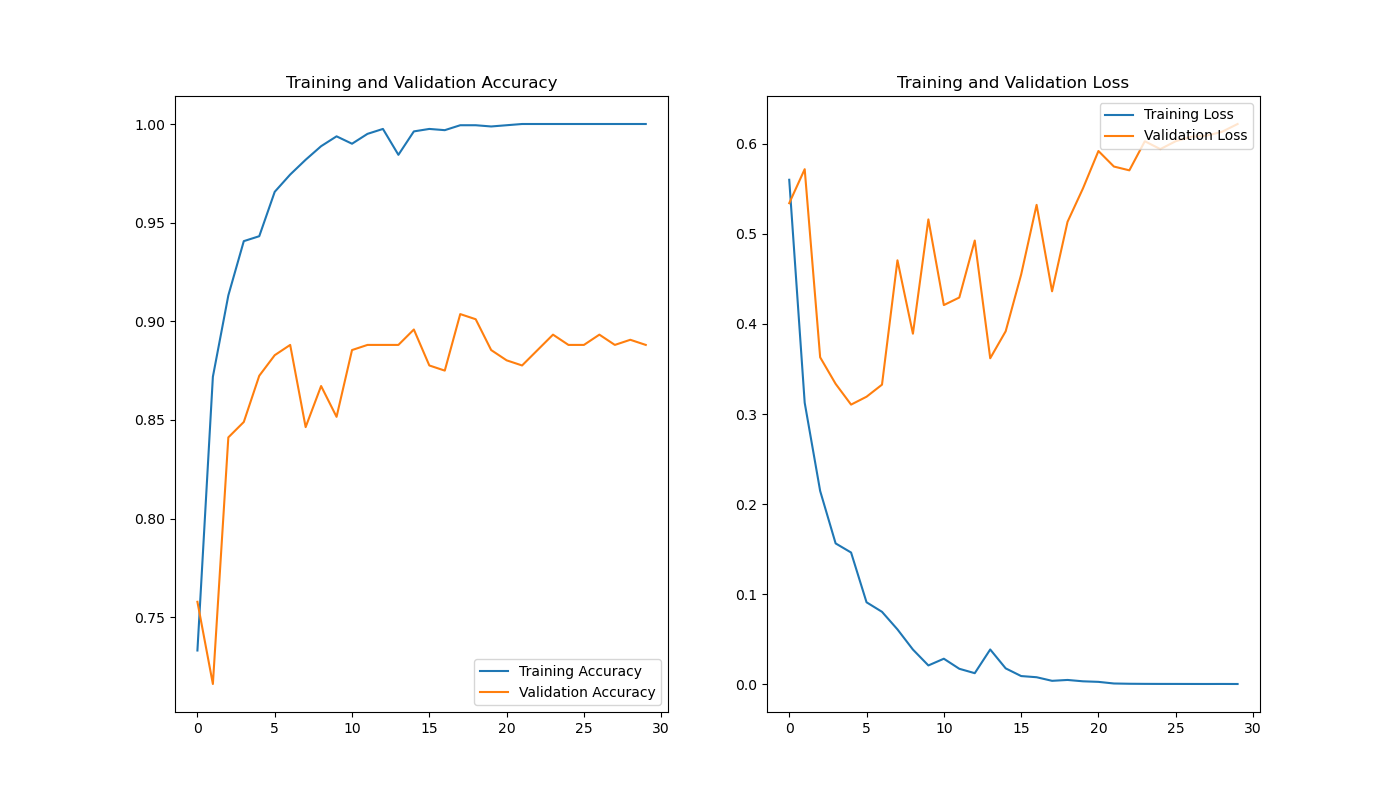
\includegraphics[width=\linewidth]{Images/baseline_curves.png}}
	\caption{Training and validation accuracy and loss for the baseline CNN over 30 epochs.}
	\label{fig:baseline_curves}
\end{figure}

\subsection{Hyperparameter Tuning}
A grid search was performed over the following hyperparameters:
\begin{itemize}
	\item Dropout rate: \{0.1, 0.2\}
	\item Initial convolutional filters: \{8, 16\}
	\item Learning rate: \{1e-3, 5e-4\}
	\item Dense units: \{256, 512\}
\end{itemize}

Early stopping restored the best weights. The best configuration achieved a validation accuracy of \textbf{0.8958} with dropout rate \textbf{0.1}, \textbf{16} filters, learning rate \(\mathbf{5\times10^{-4}}\), and \textbf{256} dense units. Full results are in Table~\ref{table:hp_results}.

\begin{table}[htbp]
	\caption{Hyperparameter Tuning Results (sorted by Val Acc)}
	\label{table:hp_results}
	\centering
	\begin{adjustbox}{width=0.48\textwidth}
		\begin{tabular}{|c|c|c|c|c|c|c|}
			\hline
			\textbf{Dropout} & \textbf{Filters} & \textbf{LR} & \textbf{Dense} & \textbf{Val Acc} & \textbf{Epoch} & \textbf{Val Loss} \\
			& & & \textbf{Units} & & & \\
			\hline
			\rowcolor{yellow}
			\bfseries 0.1 & \bfseries 16 & \bfseries 5e‑4 & \bfseries 256 & \bfseries 0.8958 & \bfseries 11 & \bfseries 0.3090 \\
			0.1 & 8  & 1e‑3 & 512 & 0.8958 &  5 & 0.2937 \\
			0.2 & 16 & 1e‑3 & 512 & 0.8880 &  4 & 0.3031 \\
			0.1 & 16 & 1e‑3 & 512 & 0.8828 &  6 & 0.2919 \\
			0.2 & 16 & 5e‑4 & 256 & 0.8828 &  8 & 0.3199 \\
			0.1 & 16 & 5e‑4 & 512 & 0.8724 &  5 & 0.3057 \\
			0.1 & 8  & 5e‑4 & 256 & 0.8724 &  5 & 0.2813 \\
			0.1 & 8  & 5e‑4 & 512 & 0.8724 &  7 & 0.3119 \\
			0.2 & 8  & 5e‑4 & 512 & 0.8698 &  8 & 0.3170 \\
			0.1 & 8  & 1e‑3 & 256 & 0.8672 &  5 & 0.3261 \\
			0.2 & 16 & 1e‑3 & 256 & 0.8672 &  8 & 0.3626 \\
			0.2 & 16 & 5e‑4 & 512 & 0.8672 & 10 & 0.3336 \\
			0.2 & 8  & 1e‑3 & 256 & 0.8646 &  6 & 0.3521 \\
			0.2 & 8  & 5e‑4 & 256 & 0.8594 & 11 & 0.3652 \\
			0.1 & 16 & 1e‑3 & 256 & 0.8385 &  6 & 0.3685 \\
			0.2 & 8  & 1e‑3 & 512 & 0.8385 &  6 & 0.3605 \\
			\hline
		\end{tabular}
	\end{adjustbox}
\end{table}

\subsection{Final Baseline Model}
Using the best hyperparameters, the model was retrained on the full training set (2,000 images) for 8 epochs. Evaluation on the held-out test set (200 images) yielded:
\begin{itemize}
	\item Test accuracy: 0.8900
	\item Test loss: 0.2772
\end{itemize}

The confusion matrix is shown in Figure~\ref{fig:conf_matrix}.

\begin{figure}[htbp]
	\centerline{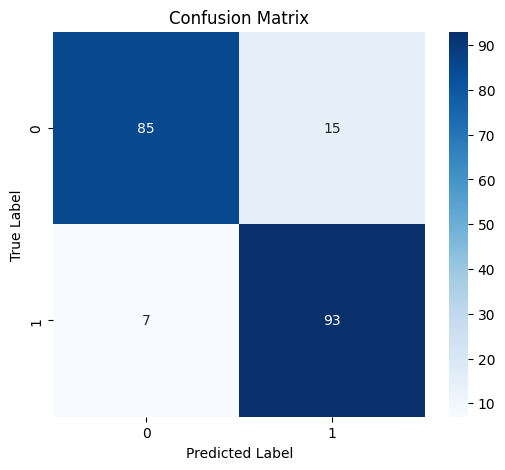
\includegraphics[width=0.7\linewidth]{Images/confusion_matrix_baseline.png}}
	\caption{Confusion matrix of the final baseline model on the test set.}
	\label{fig:conf_matrix}
\end{figure}

\subsection{Discussion}
The baseline model achieved 89\% accuracy, demonstrating strong discriminative power between COVID-19 and normal chest X-ray images. From the confusion matrix (Fig.\ref{fig:conf_matrix}), we observe:

\begin{itemize}
	\item True negatives (NORMAL correctly classified): 85
	\item False positives (NORMAL misclassified as COVID): 15
	\item False negatives (COVID misclassified as NORMAL): 7
	\item True positives (COVID correctly classified): 93
\end{itemize}

This yields a sensitivity (recall for COVID) of $93/(93+7)=0.93$ and a specificity of $85/(85+15)=0.85$. The slightly higher sensitivity indicates the model is more likely to correctly detect COVID cases, at the cost of some false alarms.  

Training curves in Fig.\ref{fig:baseline_curves} show rapid convergence of training accuracy to near 100\% within the first 10 epochs, while validation accuracy plateaus around 88\%, suggesting some overfitting that was controlled via dropout and early stopping.  

Overall, the baseline CNN provides a solid starting point;




\section{Task 3: Transfer Learning}
\section{Task 4: Explainability through Grad-CAM}
\section{Conclusions}
\section{Author contributions and collaboration}
\section{Use of Generative AI}


\subsection{Figures and Tables}
\paragraph{Positioning Figures and Tables}




\section*{References}
Example References:
\begin{thebibliography}{00}
\bibitem{b1} G. Eason, B. Noble, and I. N. Sneddon, ``On certain integrals of Lipschitz-Hankel type involving products of Bessel functions,'' Phil. Trans. Roy. Soc. London, vol. A247, pp. 529--551, April 1955.
\bibitem{b2} J. Clerk Maxwell, A Treatise on Electricity and Magnetism, 3rd ed., vol. 2. Oxford: Clarendon, 1892, pp.68--73.
\bibitem{b3} I. S. Jacobs and C. P. Bean, ``Fine particles, thin films and exchange anisotropy,'' in Magnetism, vol. III, G. T. Rado and H. Suhl, Eds. New York: Academic, 1963, pp. 271--350.
\bibitem{b4} K. Elissa, ``Title of paper if known,'' unpublished.
\bibitem{b5} R. Nicole, ``Title of paper with only first word capitalized,'' J. Name Stand. Abbrev., in press.
\bibitem{b6} Y. Yorozu, M. Hirano, K. Oka, and Y. Tagawa, ``Electron spectroscopy studies on magneto-optical media and plastic substrate interface,'' IEEE Transl. J. Magn. Japan, vol. 2, pp. 740--741, August 1987 [Digests 9th Annual Conf. Magnetics Japan, p. 301, 1982].
\bibitem{b7} M. Young, The Technical Writer's Handbook. Mill Valley, CA: University Science, 1989.
\end{thebibliography}
\end{document}
